\documentclass[a4paper,12pt]{report}
\usepackage{styles/fbe_tez}
\usepackage[utf8x]{inputenc} % To use Unicode (e.g. Turkish) characters
\renewcommand{\labelenumi}{(\roman{enumi})}
\usepackage{amsmath, amsthm, amssymb}
 % Some extra symbols
\usepackage[bottom]{footmisc}
\usepackage{cite}
\usepackage{url}
\usepackage{graphicx}
\usepackage{longtable}
\graphicspath{{figures/}} % Graphics will be here

\usepackage{multirow}
\usepackage{subfigure}
\usepackage{algorithm}
\usepackage{algorithmic}

% Added for this report
\usepackage{array}
\usepackage{tikz}
\usetikzlibrary{arrows.meta,positioning,shapes.geometric,fit,calc}
\newcommand{\cond}[1]{\texttt{#1}}
\newcolumntype{P}[1]{>{\raggedright\arraybackslash}p{#1}}
\renewcommand{\topfraction}{0.9}
\renewcommand{\bottomfraction}{0.8}
\renewcommand{\textfraction}{0.07}
\renewcommand{\floatpagefraction}{0.75}
\setcounter{topnumber}{3}
\setcounter{totalnumber}{5}
\setlength{\emergencystretch}{2em}
\usepackage{etoolbox}
% Single-spaced tables, figures and diagrams; body text keeps the template's 1.5 spacing.
\AtBeginEnvironment{table}{\linespread{1}\selectfont\renewcommand{\arraystretch}{1.3}}
\AtBeginEnvironment{figure}{\linespread{1}\selectfont}
\AtBeginEnvironment{verbatim}{\linespread{1}\selectfont}
\tikzset{
  box/.style={draw,rounded corners=2pt,align=center,font=\footnotesize,inner sep=4pt,fill=white},
  file/.style={draw,align=left,font=\footnotesize\ttfamily,inner sep=3pt,fill=gray!8},
  arr/.style={-{Stealth[length=2.2mm]},thick},
  darr/.style={-{Stealth[length=2.2mm]},thick,dashed},
}

\begin{document}

% Title Page
\title{CMPE 492 \\ Auto-Curriculum: Does a Network \\ Choose to See Blurry First?}
\author{
Ömer Faruk Çelik \\
Mustafa Taha Söylemez \\ \\
Advisor: \\
Suayb S. Arslan
}
\date{}
\maketitle{}
\pagenumbering{roman}
\tableofcontents

%======================================================================
\chapter{INTRODUCTION}
\pagenumbering{arabic}

A newborn sees the world blurry and with low contrast. Visual acuity and contrast sensitivity improve over the first months of life. One view says that this slow start is useful, not a defect: the visual system first learns coarse shape and only later fine texture, and this may make adult vision more robust to degraded input \cite{vogelsang2018}. Several studies tested this idea by training convolutional networks on a hand-made blurry-to-sharp schedule and measuring robustness \cite{vogelsang2018,jang2021blurry,arslan2024noise}. In all of them a researcher writes the schedule. Our project asks one step back: \emph{if the network chooses the blur and contrast of its own training images, based only on how fast it learns, does it start blurry and faint like an infant? And does that make it more robust?}

We use a teacher from automated curriculum learning \cite{graves2017}: a non-stationary multi-armed bandit whose arms are (blur, contrast) levels. Before each training step the teacher picks an arm, the batch is degraded at that level, and the network takes one SGD step. The reward is learning progress on the training data only. Robustness, shape bias and test data never enter the reward; we measure them only after training. If robustness were in the reward, the teacher would optimise it directly, and we could not say that an order ``emerged''. We test two hypotheses. \textbf{H1 (an infant-like order emerges):} a learning-progress teacher picks blurry, low-contrast arms early in training and sharp arms late. \textbf{H2 (robustness follows):} the self-chosen schedule gives more robustness and more shape bias than controls, including a control that sees the same arms in a shuffled order.

\textbf{Main findings} (CIFAR-10, ResNet-18, three seeds). H1 is rejected: none of the seven teacher variants we tried started blurry. With the raw learning-progress reward the teacher starts near uniform and then moves to the most degraded arm. For H2, robustness and shape bias follow \emph{exposure to blur}, not order. At 100 epochs, no ordered schedule beat a uniform random arm per batch on CIFAR-10-C. The direction of an order still matters: sharp-to-blurry is the worst order. Batch-level contrast training has almost no effect under BatchNorm; contrast is learned only with per-image mixing or GroupNorm. Table~\ref{tab:sure} grades each claim. Chapters~2--3 give the plan and related work, Chapter~4 the method, Chapters~5--7 the experiment framework as software (requirements, design, implementation and testing), Chapter~8 the results and Chapter~9 the conclusion.

\section{Broad Impact}

The project is basic research; its main value is understanding. First, it tests a popular analogy between infant vision and curriculum learning with a design that separates order from exposure. The clear negative result for H1 tells the next study that a learning-progress teacher alone does not reproduce the developmental order, and why (the reward scale favours the hardest arm). Second, the results give practical guidance for robustness training: mixing blurred images throughout training was at least as good as any ordered schedule we tested, and batch-level contrast augmentation does not work with BatchNorm. Third, the code base is public and reproducible (fixed seeds, bit-exact resume, 52 tests), so other students can extend it. We do not expect a direct product. Robustness research can, in principle, help both good and bad uses of vision systems; our small CIFAR-10 study adds almost nothing to that risk.

\section{Ethical Considerations}

We use only public benchmark data: CIFAR-10 \cite{krizhevsky2009} and CIFAR-10-C \cite{hendrycks2019}. There are no human subjects, no personal data and no data collection. The models are small image classifiers for ten object classes and are not deployed. The main cost is compute and the energy it uses: all runs together used a few hours of one cloud A100 GPU within a 300-compute-unit budget, and we kept runs short (30 and 100 epochs) and parallel to limit this. We report negative results and the limits of our evidence (three seeds, one dataset, one model) so that the claims are not stronger than the data. The repository is public and the advisor can inspect every step.

%======================================================================
\chapter{PROJECT DEFINITION AND PLANNING}

\section{Project Definition}

The project builds an experiment framework and uses it to answer H1 and H2. The data are CIFAR-10 (50\,000 training and 10\,000 test images, $32\times32$ pixels) and the model is a CIFAR-style ResNet-18 \cite{he2016resnet}. The scope covers 16 (blur, contrast) arms; two teachers, Exp3.S \cite{graves2017,auer2002} with a learning-progress reward (prediction gain and variants) and ALP-GMM \cite{portelas2019}; five controls (sharp only, random arm per batch, a hand-made blurry-to-sharp staircase, its reverse, and the teacher's own arm log shuffled in time); four measures (clean test accuracy, CIFAR-10-C split into ``seen'' and ``unseen'' corruptions, a frequency-based shape-bias proxy, and PGD adversarial accuracy); and two budgets, 30 epochs (short) and 100 epochs (full), with 3 seeds each. Chapter~\ref{ch:method} defines each part. The deliverables are the public code repository\footnote{\url{https://github.com/omarreis01/autofocus-curriculum}}, the result summaries, the experiment log, and this report.

\section{Project Planning}

\subsection{Project Time and Resource Estimation}

Table~\ref{tab:timeline} gives the actual timeline: a reading phase, a proposal, and three short experiment phases. The plan named the experiment phases F0--F8 (set-up, pipeline, teacher, controls, pilot, short budget, full budget, robustness checks, analysis).

\begin{table}[htbp]
\caption{Project timeline (2026).}
\label{tab:timeline}
\begin{center}
\small
\begin{tabular}{|l|P{10.8cm}|} \hline
\textbf{Date} & \textbf{Work} \\ \hline
Early Oct.\ -- Oct.\ 11 & Reading: Graves 2017, EfficientTrain/++, Wu 2021, Hacohen 2019, Portelas 2019 and the advisor's CCN 2024 paper. Notes in \texttt{docs/okuma/}. \\ \hline
Oct.\ 13 & Project proposal: H1/H2, seven conditions, CIFAR-10 + ResNet-18. \\ \hline
Nov.\ 3 & Set-up (F0--F4): repository, Colab launcher, degradation, training, evaluation, teacher and controls (24 tests). First GPU run: sharp, 30 epochs, 93.2\% clean. Pilot: 7 conditions, seed 0. \\ \hline
Nov.\ 4 & BatchNorm problem found and fixed (recalibration before evaluation). F5: 7 conditions $\times$ 3 seeds $\times$ 30 epochs. F6 (100 epochs) started. Extended plan written. \\ \hline
Nov.\ 8 & F6 finished. Extended code (52 tests). 13 new conditions $\times$ 3 seeds and probes on all 81 checkpoints. \\ \hline
Nov.\ 11 & Full project report (Turkish). \\ \hline
\end{tabular}
\end{center}
\end{table}

\textbf{Resources.} We used Colab Pro with a budget of 300 compute units and an A100 (40\,GB) GPU. Before any measurement, the plan estimated about 225 of the 300 units, assuming about 6\,s per epoch: F1--F2 development 15, F4 GPU comparison and pilot 10, F5 short budget (21 runs) 30, F6 full budget (21 runs) 90, F7 robustness checks 30, and a re-run reserve of 50. The real cost was much lower. One epoch takes 2.0\,s in eager mode (\texttt{torch.compile} gives 1.7\,s but costs 30\,s to compile, so we did not use it). A full CIFAR-10-C evaluation takes 15\,s. Because all data stays in GPU memory, 6 runs share one A100 in parallel; one wave of 12 parallel runs ran out of memory (Table~\ref{tab:risk}). Teacher runs need one extra forward pass per step for the reward.

\subsection{Success Criteria}

We set five criteria before the experiments; all were met. (i)~\emph{Pipeline is correct:} the sharp condition reaches about 93\% clean accuracy after 30 epochs (known value for ResNet-18); result: 93.2\%. (ii)~\emph{Teacher is sane:} with a network that does not learn, the teacher gives no reward and stays uniform; with one arm that pays more, it concentrates on that arm (both are unit tests). (iii)~\emph{Fair comparison:} every condition uses the same number of steps, the same learning-rate schedule and the same data order (tested). (iv)~\emph{Statistics:} every reported number is the mean $\pm$ standard deviation over 3 seeds, at a short and a full budget. (v)~\emph{A clear answer:} the report answers H1 and H2 either way, with evidence for each claim; a negative result counts as a result.

\subsection{Risk Analysis}
\label{sec:risk}

Table~\ref{tab:risk} lists the risks we planned for and the problems that happened.

\begin{table}[htbp]
\caption{Risks, mitigations and what happened.}
\label{tab:risk}
\begin{center}
\footnotesize
\begin{tabular}{|P{3.6cm}|P{5.0cm}|P{5.3cm}|} \hline
\textbf{Risk} & \textbf{Mitigation} & \textbf{What happened} \\ \hline
Gains come from blur exposure, not order \cite{wu2021curricula,katzhendler2019} & Shuffled control (same arms, random order), random and reverse controls & This was the key control; see Chapter~8. \\ \hline
Colab session ends during a run & Checkpoint every 5 epochs to Google Drive, bit-exact \texttt{--resume} & Happened in F6 (the PC was shut down near epoch 40); runs resumed. \\ \hline
A100 not available / budget overrun & Measure speed first (F4), keep runs short & A100 was available; measured cost far below estimate. \\ \hline
Slow dataset servers & Hugging Face mirrors, checked against the official files (CIFAR-10 archive by MD5; CIFAR-10-C label order against the official test labels) & Zenodo and Toronto were very slow; mirrors took $\sim$1.5\,min. \\ \hline
Bandit does not move in 3k--10k steps & Larger learning rate $\eta$ & With Graves' $\eta=10^{-3}$ the policy did not move; we use $\eta=0.01$. \\ \hline
Hidden bug in a mixed-arm pipeline & Pilot run before the main runs & BatchNorm mismatch found in the pilot (Chapter~\ref{ch:method}). \\ \hline
GPU out of memory & Fewer parallel runs & 3 of 12 parallel runs (GroupNorm and per-image) died; re-run from checkpoint at 6 parallel (\texttt{colab/finish\_ext.sh}). Same set-up, so results are not affected. \\ \hline
Small effects & 3 seeds, two budgets, report std & Most differences are far above the std; the small ones are marked. \\ \hline
\end{tabular}
\end{center}
\end{table}

\subsection{Team Work (if applicable)}

The team has two members. For the reading phase, the work was split by topic: Ömer Faruk Çelik read the curriculum and bandit papers (Graves 2017, EfficientTrain/++, Wu 2021, Hacohen 2019, Portelas 2019) and wrote that part of the reading notes; the other topics of the reading notes were assigned to Mustafa Taha Söylemez. Both read the advisor's CCN 2024 paper. The repository history shows that Ömer Faruk Çelik wrote the code and ran the experiments. The advisor, Suayb S.\ Arslan, gave the research direction through his work on developmental noise and resolution schedules \cite{arslan2024noise}.

%======================================================================
\chapter{RELATED WORK}

\textbf{Automated curriculum with bandits.} Graves et al.\ \cite{graves2017} let a non-stationary bandit, Exp3.S \cite{auer2002}, choose which task to sample next. The reward is learning progress, for example the prediction gain (PG): the drop in loss on a batch after one update. They found that uniform sampling over tasks is a strong baseline, and warned that PG can favour arms with high gradient variance. We use this teacher directly, with image degradation levels as arms instead of tasks. Portelas et al.\ \cite{portelas2019} proposed ALP-GMM, which fits a Gaussian mixture over a continuous task space and samples where the absolute learning progress is high; it is our second teacher.

\textbf{Low-frequency-first training.} EfficientTrain \cite{wang2023efficienttrain} and EfficientTrain++ \cite{wang2024efficienttrainpp} show the network low-frequency content first and the full image later. This speeds up ImageNet training by about 1.5--3$\times$ without accuracy loss. This is the closest prior work, but the schedule is found offline and then fixed, the goal is compute, and robustness is not measured. Our hand-made staircase is a version of this fixed schedule.

\textbf{When do curricula help?} Wu, Dyer and Neyshabur \cite{wu2021curricula} trained thousands of models and found that curriculum, anti-curriculum and random order give the same result in standard training; small gains come from pacing, and curricula help mainly with short budgets or noisy labels. This is the main reason for our shuffled, random and reverse controls and for the two budgets. Hacohen and Weinshall \cite{hacohen2019} split a curriculum into a scoring function and a pacing function, and report small gains (1--2 points) from easy-to-hard order. In our design one bandit sets both order and pacing, so we keep the learning-rate schedule the same in every condition.

\textbf{Developmental vision and blur.} Vogelsang et al.\ \cite{vogelsang2018} argue that initially poor acuity may be adaptive and support this with networks trained blurry-to-sharp. Katzhendler and Weinshall \cite{katzhendler2019} replied that low-resolution images could simply be mixed in at all times; the benefit may come from exposure, not order. Jang and Tong \cite{jang2021blurry} found that for objects (unlike faces) the robustness from blurry-to-clear training is not kept at the end of training; later \cite{jang2024blur} they showed that training with mixed blur gives networks more shape sensitivity and more robustness to noise. Arslan, Jang and Sinha \cite{arslan2024noise} showed that decreasing internal neural noise from high to low during training, and low-to-high resolution, improves robustness to degraded input. All of these schedules are set by hand (Table~\ref{tab:related}). Our question is whether the order appears when the network chooses. Contrast is our addition.

\textbf{Robustness, shape and normalisation.} CIFAR-10-C \cite{hendrycks2019} applies 19 corruptions at 5 severities to the CIFAR-10 test set. Geirhos et al.\ \cite{geirhos2019} defined shape bias with style-transfer cue-conflict images; we use a simpler frequency proxy because that set does not fit $32\times32$ images. Wang et al.\ \cite{wang2020highfreq} showed that CNNs use high-frequency components that humans cannot see, which motivates our low-/high-pass probes. PGD \cite{madry2018} is the standard iterative adversarial attack. BatchNorm \cite{ioffe2015} normalises with batch statistics in training and with running averages at test time; GroupNorm \cite{wu2018gn} normalises within each sample and has no batch statistics. This difference turned out to be central for contrast (Chapter~\ref{ch:method}).

\begin{table}[htbp]
\caption{Position of this project relative to the closest work.}
\label{tab:related}
\begin{center}
\footnotesize
\begin{tabular}{|P{3.4cm}|P{3.2cm}|P{3.4cm}|P{3.6cm}|} \hline
\textbf{Work} & \textbf{Who sets the order} & \textbf{Axis} & \textbf{Measures robustness?} \\ \hline
Graves et al.\ \cite{graves2017} & Bandit, learning progress & Tasks (text, bAbI) & No \\ \hline
EfficientTrain/++ \cite{wang2023efficienttrain,wang2024efficienttrainpp} & Offline search, then fixed & Frequency, augmentation & No \\ \hline
Vogelsang; Jang \& Tong \cite{vogelsang2018,jang2021blurry,jang2024blur} & Researcher & Blur & Yes \\ \hline
Arslan et al.\ \cite{arslan2024noise} & Researcher & Internal noise, resolution & Yes (noisy input) \\ \hline
\textbf{This project} & \textbf{Bandit, learning progress} & \textbf{Blur and contrast} & \textbf{Yes (CIFAR-10-C, PGD, shape proxy)} \\ \hline
\end{tabular}
\end{center}
\end{table}

%======================================================================
\chapter{METHODOLOGY}
\label{ch:method}

\textbf{Data, model and training.} We train on CIFAR-10 with random crop (padding 4) and horizontal flip. Blur and contrast are applied on the GPU after augmentation. The model is ResNet-18 in its CIFAR form ($3\times3$ stem, no max-pool) with BatchNorm; one group of experiments uses GroupNorm with 32 groups. We use SGD with Nesterov momentum 0.9, weight decay $5\cdot10^{-4}$, batch size 512 and bf16 mixed precision. The learning rate rises linearly to 0.2 over the first 15\% of steps and then follows a cosine to zero; this schedule is the same in every condition. The short budget is 30 epochs (2\,910 steps) and the full budget is 100 epochs (9\,700 steps), with 97 steps per epoch. Every condition runs with seeds 0, 1 and 2.

\textbf{Arms: blur and contrast.} An arm is a pair $(\sigma, c)$ from a grid of 4 blur levels ($\sigma\in\{0, 0.75, 1.5, 3\}$ pixels) $\times$ 4 contrast levels ($c\in\{1, 0.6, 0.35, 0.2\}$) = 16 arms; the arm $(0,1)$ is the sharp image. Blur is a separable Gaussian filter with standard deviation $\sigma$ pixels and reflect padding. Contrast then moves every pixel toward the image mean $m$ of its channel, $x' = m + c\,(x - m)$. In all conditions except one (\cond{random\_image}), every image in a batch gets the same arm.

\textbf{Teacher: Exp3.S with learning-progress rewards.} At step $t$ the teacher keeps weights $w_i$ for the $K=16$ arms and samples arm $a_t$ from
\begin{equation}
\pi_t(i) = (1-\epsilon)\,\frac{e^{w_i}}{\sum_j e^{w_j}} + \frac{\epsilon}{K}.
\end{equation}
The batch is degraded with arm $a_t$, the network takes one SGD step, and the teacher measures a raw reward $\tilde r_t$. \textbf{PG} (prediction gain) is the loss on the same batch before the update minus the loss after it (one extra forward pass). \textbf{SPG} is the same difference on a fresh batch from the same arm; it removes the bias of measuring on the batch just trained on. \textbf{RPG} (relative PG) is PG divided by the loss before the update; it removes the scale of the loss. The raw reward is mapped to $[-1,1]$ with the 20th and 80th percentiles $q^{lo}, q^{hi}$ of the last 1000 raw rewards \cite{graves2017}:
\begin{equation}
r_t = \operatorname{clip}\!\left(2\,\frac{\tilde r_t - q^{lo}}{q^{hi}-q^{lo}} - 1,\; -1,\; 1\right).
\end{equation}
The Exp3.S update with importance weighting is $w_{a_t} \leftarrow w_{a_t} + \eta\, r_t / \pi_t(a_t)$, followed by weight sharing with rate $\alpha_t = 1/t$ so that the teacher can track a changing best arm. We use $\eta=0.01$, $\epsilon=0.05$. Graves et al.\ use $\eta=10^{-3}$ for about $10^5$ steps; with our 3k--10k steps it did not move the policy (Table~\ref{tab:risk}). The forward passes that measure the reward do not change the BatchNorm running statistics, so a teacher run differs from a fixed-arm run only in the choice of arms.

\textbf{ALP-GMM.} The second teacher samples a continuous point in the $(\sigma, c)$ box (scaled to $[0,1]^2$), with 20\% random samples and otherwise from a Gaussian mixture fitted every 250 steps on the absolute learning progress. Each sample is rounded to the nearest of the 16 arms for training.

\textbf{Conditions.} Table~\ref{tab:conditions} lists the 20 conditions: the seven main ones ran at both budgets, the 13 extended ones at 30 epochs only.

\begin{table}[htbp]
\caption{Conditions and the question each one answers.}
\label{tab:conditions}
\begin{center}
\footnotesize
\renewcommand{\arraystretch}{1.1}
\begin{tabular}{|l|P{5cm}|P{4.3cm}|} \hline
\textbf{Condition} & \textbf{What it does} & \textbf{What it tests} \\ \hline
\multicolumn{3}{|l|}{\textit{Main seven (30 and 100 epochs)}} \\ \hline
\cond{sharp} & Always $(0, 1)$. & Lower bound: no blur seen. \\
\cond{random} & Uniform random arm per batch. & Exposure without order. \\
\cond{staircase} & Diagonal $(3,.2)\to(1.5,.35)\to(.75,.6)\to(0,1)$ in 4 equal stages over the first 50\% of steps, then sharp. & Hand-made blurry-to-sharp (what H1 expects). \\
\cond{reverse} & Staircase reversed in time; same arm counts. & Does the direction matter? \\
\cond{teacher\_pg} & Exp3.S + PG. & Main method. \\
\cond{teacher\_spg} & Exp3.S + SPG. & Same-batch bias of PG. \\
\cond{shuffled} & Arm log of \cond{teacher\_pg} (same seed), shuffled in time. & Same exposure, no order. \\ \hline
\multicolumn{3}{|l|}{\textit{A: teacher variants (30 epochs)}} \\ \hline
\cond{teacher\_rpg} & Exp3.S + RPG. & Is ``hard first'' caused by the PG scale? \\
\cond{teacher\_pg\_eta0.003/0.03} & $\eta\times0.3$ and $\times3$. & Sensitivity to $\eta$. \\
\cond{teacher\_pg\_noiw} & No importance weighting. & Update detail. \\
\cond{teacher\_alp} & ALP-GMM. & Does another teacher choose the same? \\ \hline
\multicolumn{3}{|l|}{\textit{B: training regime (30 epochs)}} \\ \hline
\cond{random\_image} & Random arm per image (mixed batch). & Per batch vs per image. \\
\cond{sharp/random/teacher\_pg\_gn} & GroupNorm(32) instead of BatchNorm. & Do results depend on BatchNorm? \\
\cond{random\_blur} & Blur axis only ($c=1$). & Which axis gives robustness? \\
\cond{random\_contrast} & Contrast axis only ($\sigma=0$). & Same question. \\
\cond{staircase\_f025/f075} & Staircase over 25\% / 75\% of steps. & Length of the hand-made schedule. \\ \hline
\end{tabular}
\end{center}
\end{table}

\textbf{Measures.} \textbf{Clean} is CIFAR-10 test accuracy. \textbf{CIFAR-10-C} \cite{hendrycks2019} has 19 corruptions $\times$ 5 severities. \emph{Seen} is the mean over the 6 corruptions close to our training degradations (Gaussian, defocus, glass, motion and zoom blur, contrast); \emph{unseen} is the mean over the other 13 (noise, weather, digital). We also report the mean of the 4 noise corruptions and the contrast corruption alone. \textbf{Shape bias (CIFAR proxy):} a hybrid image is the low-frequency part (Gaussian $\sigma=2$) of an image of class A plus the high-frequency part of an image of class B; shape bias is the share of A answers among A or B answers, over about 10\,000 pairs. This is not Geirhos' style-transfer test \cite{geirhos2019}; it measures reliance on low versus high frequencies. We also report accuracy on high-pass images ($\sigma=1$). \textbf{PGD-10} \cite{madry2018} uses $L_\infty$, $\epsilon=1/255$, step $\epsilon/4$, random start, on 2\,000 test images. We also measured FGSM but do not use it, because it looks gradient-masked: at 100 epochs, \cond{sharp} scores higher under FGSM at $2/255$ than under PGD at $1/255$ (53.6 vs 44.9).

\textbf{BatchNorm recalibration.} In the pilot, \cond{sharp} was normal, but every condition that mixes arms over time scored only 13--60\% clean accuracy. The cause is BatchNorm. Each batch comes from one arm. In training, BatchNorm uses the statistics of the current batch, so this is fine. At test time it uses running averages, which are a mix of degraded batches and do not fit clean images. We tested this: after recomputing the running statistics on 100 batches of clean \emph{training} images, \cond{random} rose from 60 to 89.1\% and \cond{teacher\_spg} from 16 to 87.2\%, while \cond{sharp} did not change. We therefore recalibrate BatchNorm this way before every evaluation and probe. No test data is used.

The same mechanism acts during training. When a whole batch has contrast $c$, the first BatchNorm layer largely removes the change of scale, so the network hardly ``sees'' low contrast. This is an explanation; Chapter~8 (``Which axis and which regime?'') gives the experiments that support it.

%======================================================================
\chapter{REQUIREMENTS SPECIFICATION}

The ``system'' is the experiment framework. Its one actor is the researcher, who configures a condition (\texttt{make\_configs}), trains with a schedule or teacher (\texttt{train}), resumes from a checkpoint (extends training), evaluates clean and CIFAR-10-C accuracy (\texttt{eval}), probes shape bias, filters and PGD (\texttt{probe}), and aggregates and plots (\texttt{collect}, \texttt{digest}). Its one external system is the Colab A100 runtime with Google Drive, used by training, evaluation and probing. Table~\ref{tab:req} lists the requirements.

\begin{table}[htbp]
\caption{Functional and non-functional requirements.}
\label{tab:req}
\begin{center}
\footnotesize
\renewcommand{\arraystretch}{1.0}
\begin{tabular}{|l|P{8.1cm}|P{5.0cm}|} \hline
\textbf{ID} & \textbf{Requirement} & \textbf{Where / how it is checked} \\ \hline
FR1 & Degrade a batch with any arm $(\sigma, c)$ on the GPU; arm $(0,1)$ is the identity. & \texttt{degrade.py} \\
FR2 & Run any of the 20 conditions from one JSON config (condition, seed, budget). & \texttt{make\_configs.py}, \texttt{schedule.py} \\
FR3 & Teacher: Exp3.S with PG, SPG or RPG reward; ALP-GMM as an option. & \texttt{teacher.py}, \texttt{teacher\_alp.py} \\
FR4 & Log the arm of every step and, for teachers, the rewards and policies. & \texttt{arms.npy}, \texttt{teacher.npz} \\
FR5 & Replay a teacher arm log shuffled in time (\cond{shuffled}). & \texttt{schedule.py} \\
FR6 & Evaluate clean accuracy and all 19$\times$5 CIFAR-10-C sets, with seen/unseen means. & \texttt{eval.py} \\
FR7 & Probe hybrid shape bias, low-/high-pass accuracy, FGSM and PGD. & \texttt{probe.py} \\
FR8 & Aggregate all seeds into mean $\pm$ std summaries and per-epoch curves. & \texttt{collect.py}, \texttt{digest.py}, \texttt{blur\_curve.py} \\ \hline
NFR1 & \textbf{Determinism:} same config and seed give the same arm sequence and data order. & Per-epoch seeded generators; condition tests. \\
NFR2 & \textbf{Bit-exact resume:} a run stopped and resumed equals an uninterrupted run. & \texttt{test\_resume.py} for every schedule type. \\
NFR3 & \textbf{Fairness:} same steps, same LR schedule and same data order in all conditions. & One training loop; LR is a function of the step only. \\
NFR4 & \textbf{Reward measurement is side-effect free:} it does not change BatchNorm statistics or training. & \texttt{test\_teacher.py}. \\
NFR5 & \textbf{No test-data leakage:} rewards use training data; BN recalibration uses clean training images. & Code review; \texttt{eval.py}. \\
NFR6 & \textbf{Budget and time:} a 30-epoch run in minutes on one A100; stay within 300 compute units. & 2.0\,s/epoch measured; 6 runs in parallel. \\
NFR7 & \textbf{Robust to session loss:} checkpoints every 5 epochs, written atomically to Drive. & F6 was interrupted and resumed. \\
NFR8 & \textbf{Testable without a GPU:} CPU smoke run with fake data. & \texttt{python -m src.smoke --fake-data}. \\ \hline
\end{tabular}
\end{center}
\end{table}

%======================================================================
\chapter{DESIGN}

\section{Information Structure}

The framework has no database. Its information lives in files with a fixed layout (Table~\ref{tab:files}): one JSON config per run, one result folder per run under \texttt{results/<budget>/<condition>/<seed>/} (written by \texttt{train}), and one summary per budget (written by \texttt{collect}).

\begin{table}[htbp]
\caption{Files of the framework.}
\label{tab:files}
\begin{center}
\footnotesize
\renewcommand{\arraystretch}{1.05}
\begin{tabular}{|P{4.9cm}|P{9.3cm}|} \hline
\textbf{File} & \textbf{Content} \\ \hline
\texttt{configs/<short|full>/}\newline\texttt{<condition>\_s<seed>.json} & One run: \texttt{condition}, \texttt{seed}, \texttt{epochs}, \texttt{norm}, \texttt{signal}, \texttt{eta}, \texttt{importance}, \texttt{staircase\_frac}, \texttt{arms\_path}, \ldots{} A \cond{shuffled} config points (\texttt{arms\_path}) to the \texttt{arms.npy} of the \cond{teacher\_pg} run with the same seed. \\ \hline
\multicolumn{2}{|l|}{\textit{In \texttt{results/<budget>/<condition>/<seed>/}}} \\ \hline
\texttt{last.pt} & Checkpoint: model, optimiser, grad scaler, schedule state (bandit weights, RNG state, reward buffer), arm log, epoch, config. \\
\texttt{metrics.jsonl} & One row per epoch: \texttt{epoch}, \texttt{train\_loss}, \texttt{test\_acc}, \texttt{sec}. \\
\texttt{arms.npy} & Arm index (0--15) of every training step; arm $= 4\,i_\sigma + i_c$. \\
\texttt{teacher.npz} & Teacher runs only: raw reward per step and the 16-arm policy per step. \\
\texttt{eval.json} & \texttt{clean}, accuracy per corruption and severity, \texttt{seen\_mean}, \texttt{unseen\_mean}, \texttt{all\_mean}. \\
\texttt{probe.json} & Low-/high-pass accuracy per $\sigma$, hybrid shape bias per $\sigma$, FGSM and PGD-10 per $\epsilon$. \\ \hline
\texttt{results/}\newline\texttt{<budget>\_summary.json} & Mean and std over seeds for every condition and metric. \\ \hline
\end{tabular}
\end{center}
\end{table}

\section{Information Flow}

Figure~\ref{fig:flow} shows one training step; the schedule is a fixed sequence or a teacher, and fixed schedules ignore the update. After training, the evaluation pipeline runs on the last checkpoint: \texttt{last.pt} $\to$ recalibrate BN on 100 clean training batches $\to$ \texttt{eval} (clean + CIFAR-10-C) and \texttt{probe} (hybrids, filters, PGD) $\to$ \texttt{collect} (mean $\pm$ std).

\begin{figure}[htbp]
\centering
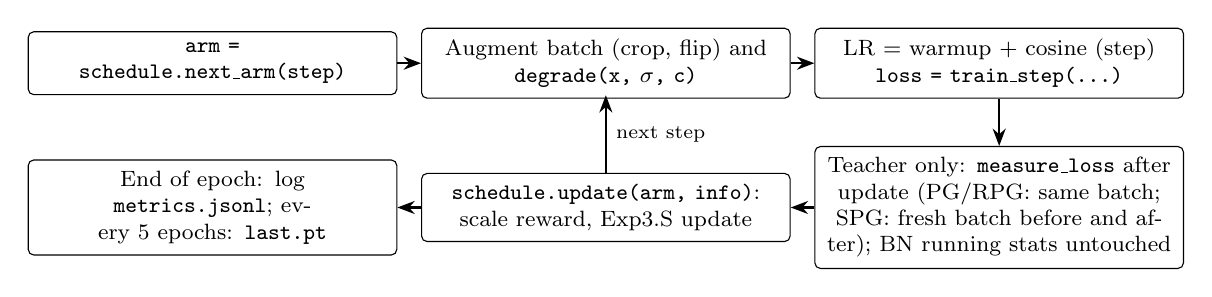
\begin{tikzpicture}[node distance=0.35cm and 0.3cm, b/.style={box,text width=4.4cm}]
\node[b] (a) {\texttt{arm =}\\\texttt{schedule.next\_arm(step)}};
\node[b,right=of a] (b) {Augment batch (crop, flip) and\\\texttt{degrade(x, $\sigma$, c)}};
\node[b,right=of b] (c) {LR $=$ warmup + cosine (step)\\\texttt{loss = train\_step(...)}};
\node[b,below=0.6cm of c] (d) {Teacher only: \texttt{measure\_loss} after update (PG/RPG: same batch; SPG: fresh batch before and after); BN running stats untouched};
\node[b,left=of d] (e) {\texttt{schedule.update(arm, info)}: scale reward, Exp3.S update};
\node[b,left=of e] (f) {End of epoch: log \texttt{metrics.jsonl}; every 5 epochs: \texttt{last.pt}};
\draw[arr] (a)--(b); \draw[arr] (b)--(c); \draw[arr] (c)--(d); \draw[arr] (d)--(e); \draw[arr] (e)--(f);
\draw[arr] (e.north) -- node[right,font=\scriptsize]{next step} (e.north |- a.south);
\end{tikzpicture}

\caption{One training step. Only teacher schedules use the reward branch.}
\label{fig:flow}
\end{figure}

\section{System Design}

{\sloppy Figure~\ref{fig:modules} shows the modules of \texttt{src/} and their dependencies. \texttt{train.py} is the centre. It builds the model, gets a schedule from \texttt{schedule.make\_schedule}, and calls \texttt{degrade} on each batch. All schedules share one small interface (\texttt{Schedule}): \texttt{next\_arm(step)}, \texttt{update(arm, info)}, \texttt{state\_dict}/\texttt{load\_state\_dict} for resume, and \texttt{save}. Teachers declare which reward measurements they need (\texttt{wants\_loss\_after}, \texttt{wants\_fresh\_batch}); \cond{random\_image} declares \texttt{per\_image}. So the training loop has no condition-specific branches.\par}

\begin{figure}[htbp]
\centering
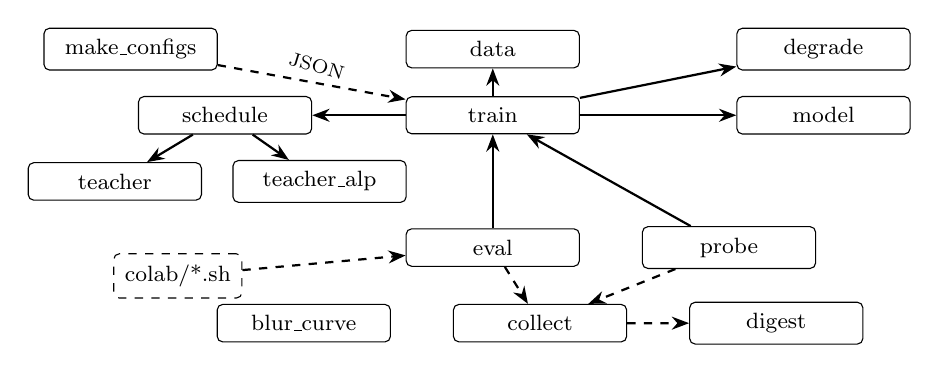
\begin{tikzpicture}[m/.style={box,minimum width=2.2cm},yscale=0.6]
\node[m] (cfg) at (-4.6,2.2) {make\_configs};
\node[m] (data) at (0,2.2) {data};
\node[m] (deg) at (4.2,2.2) {degrade};
\node[m] (sched) at (-3.4,0.8) {schedule};
\node[m] (train) at (0,0.8) {train};
\node[m] (model) at (4.2,0.8) {model};
\node[m] (teach) at (-4.8,-0.6) {teacher};
\node[m] (alp) at (-2.2,-0.6) {teacher\_alp};
\node[m] (eval) at (0,-2.0) {eval};
\node[m] (probe) at (3.0,-2.0) {probe};
\node[box,dashed] (colab) at (-4.0,-2.6) {colab/*.sh};
\node[m] (curve) at (-2.4,-3.6) {blur\_curve};
\node[m] (collect) at (0.6,-3.6) {collect};
\node[m] (digest) at (3.6,-3.6) {digest};
\draw[arr] (train)--(sched); \draw[arr] (sched)--(teach); \draw[arr] (sched)--(alp);
\draw[arr] (train)--(model); \draw[arr] (train)--(deg); \draw[arr] (train)--(data);
\draw[arr] (eval)--(train); \draw[arr] (probe)--(train);
\draw[darr] (cfg) -- node[above,font=\scriptsize,sloped]{JSON} (train);
\draw[darr] (eval)--(collect); \draw[darr] (probe)--(collect);
\draw[darr] (collect)--(digest);
\draw[darr] (colab) -- (eval);
\end{tikzpicture}
\caption{Module diagram of \texttt{src/}. Solid: Python import. Dashed: data files or script calls. The Colab scripts call \texttt{train}, \texttt{eval} and \texttt{probe}; \texttt{blur\_curve} reads \texttt{arms.npy}.}
\label{fig:modules}
\end{figure}

\section{User Interface Design (if applicable)}

Not applicable: the project has no user interface; the researcher uses command-line modules and Colab cells.

%======================================================================
\chapter{IMPLEMENTATION AND TESTING}

\section{Implementation}

The code is Python with PyTorch, about 1\,200 lines in 14 modules in \texttt{src/} and about 340 lines of tests. \textbf{GPU-resident data:} the whole CIFAR-10 training set is a \texttt{uint8} tensor on the GPU, and augmentation, blur and contrast run there; there is no CPU data loader. \textbf{Reproducible randomness:} each epoch uses a generator seeded by (seed, epoch) for data order and augmentation; SPG draws its fresh batch from a second, separate stream, so the training data order matches every other condition. \textbf{Side-effect-free reward:} \texttt{measure\_loss} runs a train-mode forward pass with \texttt{track\_running\_stats} turned off, so measuring the reward does not change BatchNorm statistics; the only GPU synchronisation per step is reading the raw reward. \textbf{Resumable runs:} the checkpoint (Table~\ref{tab:files}) is written to a temporary file and renamed (atomic write); metrics rows after the restored epoch are dropped. \textbf{Stable bandit:} Exp3.S keeps log-weights normalised to a maximum of 0, so the exponentials do not overflow over long runs. Table~\ref{tab:risk} gives the problems met and their fixes.

\section{Testing}

\textbf{Unit and integration tests:} \texttt{pytest} runs 52 test cases (20 test functions, several parametrised over conditions) on the CPU in about 30\,s (Table~\ref{tab:tests}); the last local run gave \texttt{52 passed in 28.59s}. \textbf{Smoke test:} \texttt{python -m src.smoke --fake-data} runs train, eval and probe end to end on random data on the CPU; on Colab the same command checks the real data. \textbf{Acceptance runs:} the first GPU run (\cond{sharp}, 30 epochs, seed 0) reached 93.2\% clean accuracy (Section~2.2.2); the 7-condition pilot (seed 0) checked every condition on the GPU and exposed the BatchNorm problem before the main runs.

\begin{table}[htbp]
\caption{Automated tests.}
\label{tab:tests}
\begin{center}
\footnotesize
\renewcommand{\arraystretch}{1.0}
\begin{tabular}{|l|P{11cm}|} \hline
\textbf{File} & \textbf{What is checked} \\ \hline
\texttt{test\_degrade.py} & Sharp arm is the identity; contrast keeps the channel mean and scales the std by $c$; blur removes more high-frequency energy as $\sigma$ grows; arm index mapping; augmentation is a padded crop or its mirror; per-image degradation equals degrading each image with its own arm. \\
\texttt{test\_teacher.py} & Reward measurement does not change training; a network that does not learn gives no reward and a uniform policy (PG and SPG); the teacher concentrates on an arm with higher reward and stays near uniform when all arms pay alike; ALP-GMM concentrates on an arm with steady progress. \\
\texttt{test\_conditions.py} & Every condition gives a valid arm at every step; staircase goes blurry to sharp and reverse mirrors it; shuffled replays the teacher's arm counts in a new order; axis ablations draw only their axis; \cond{random\_image} mixes arms in a batch and is seeded. \\
\texttt{test\_probe.py} & Hybrid bias follows the frequency band a model reads; attacks stay in the $\epsilon$-box and hurt only with budget; the probe reports every measure on fake data. \\
\texttt{test\_resume.py} & A run stopped and resumed matches an uninterrupted run, for every schedule type. \\ \hline
\end{tabular}
\end{center}
\end{table}

\section{Deployment}

The code is written and tested (CPU) on a laptop and pushed to the public GitHub repository. Colab Pro is only a launcher: it clones the repository, downloads CIFAR-10 and CIFAR-10-C from Hugging Face, and runs shell scripts in the background (\texttt{nohup}) on the A100. Checkpoints and JSON results go to Google Drive (\texttt{results/}, \texttt{logs/}), so runs survive a closed browser tab and resume after a lost runtime. \texttt{docs/report/make\_figures.py} makes this report's figures and tables from the result summaries. Commands on Colab (after mounting Drive), then local CPU tests:\par
{\footnotesize
\begin{verbatim}
git clone https://github.com/omarreis01/autofocus-curriculum.git
cd autofocus-curriculum && pip install -q -r requirements.txt
python -m src.data --data-dir /content/data      # ~1.5 min
python -m src.smoke --data-dir /content/data
bash colab/run_budget.sh short 0 1 2             # 7 conditions, 30 epochs
bash colab/run_budget.sh full 0 1 2              # 7 conditions, 100 epochs
bash colab/run_conds.sh short 6 "0 1 2" teacher_rpg teacher_alp ...
python -m src.collect --results $D/results/short --epochs 30 \
    > $D/results/short_summary.json
uv venv --python 3.13 .venv
uv pip install --python .venv/bin/python torch torchvision \
    --index-url https://download.pytorch.org/whl/cpu
uv pip install --python .venv/bin/python -r requirements.txt
.venv/bin/python -m pytest -q tests
\end{verbatim}
}

%======================================================================
\chapter{RESULTS}

All numbers are accuracies in \%, as the mean $\pm$ std over 3 seeds; ``C'' means CIFAR-10-C. Tables~\ref{tab:full30} and \ref{tab:full100} in the appendix give every condition and measure, with std.

\textbf{Main comparison at 100 epochs.} Figure~\ref{fig:main} places the seven main conditions by clean and CIFAR-10-C accuracy. \cond{random} is the best on C: 85.3 seen and 84.4 unseen, with clean accuracy (92.2) only 2.6 points below \cond{sharp}. The teachers (\cond{teacher\_pg}, \cond{teacher\_spg}) and \cond{shuffled} stay at 85--87 clean, because they spend most of training on the most degraded arm (Figure~\ref{fig:worst}). \cond{staircase} ends close to \cond{sharp} (93.1 clean, 77.0 / 78.8 on C): after the blurry phase, the model adapts back to sharp images. \cond{reverse} is good on C-seen (80.9) but the worst on C-unseen (71.9). At 30 epochs the ranking is the same (Table~\ref{tab:full30}).

\begin{figure}[htbp]
\centering
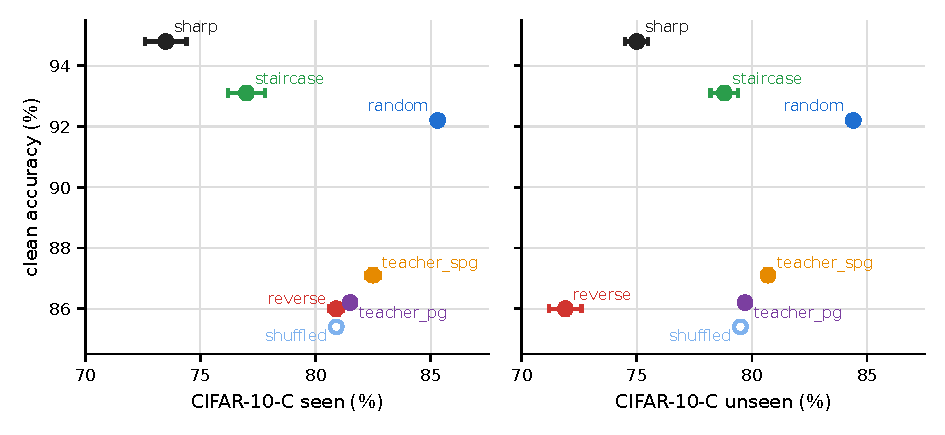
\includegraphics[width=\textwidth]{main_100ep.pdf}
\caption{Clean vs CIFAR-10-C accuracy at 100 epochs: \cond{random} is best on corruptions and loses little clean accuracy. Bars are $\pm$ std (mostly smaller than the dots); axes do not start at zero.}
\label{fig:main}
\end{figure}

\textbf{Does the teacher start blurry, and where does it go?} This is the direct test of H1. Figure~\ref{fig:curves} shows the mean blur $\sigma$ and mean contrast of the batches trained in each epoch. If H1 were true, a teacher curve would look like the staircase: high $\sigma$ and low $c$ at the start, then sharp. The dotted line is the expected value of uniform choice ($\sigma=1.31$, $c=0.54$). None of the teachers starts blurry; all start near uniform. With raw PG and SPG the teacher moves to \emph{more} blur and \emph{less} contrast over time. RPG and ALP-GMM stay near uniform. With $\eta=0.03$ the teacher reaches the most degraded arm fast and returns towards uniform in the last third; this is not a blurry start either. At 100 epochs the pattern is the same over a longer time: \cond{teacher\_pg} stays in the most degraded region from about epoch 10 to 70 and then partly returns.

\begin{figure}[htbp]
\centering
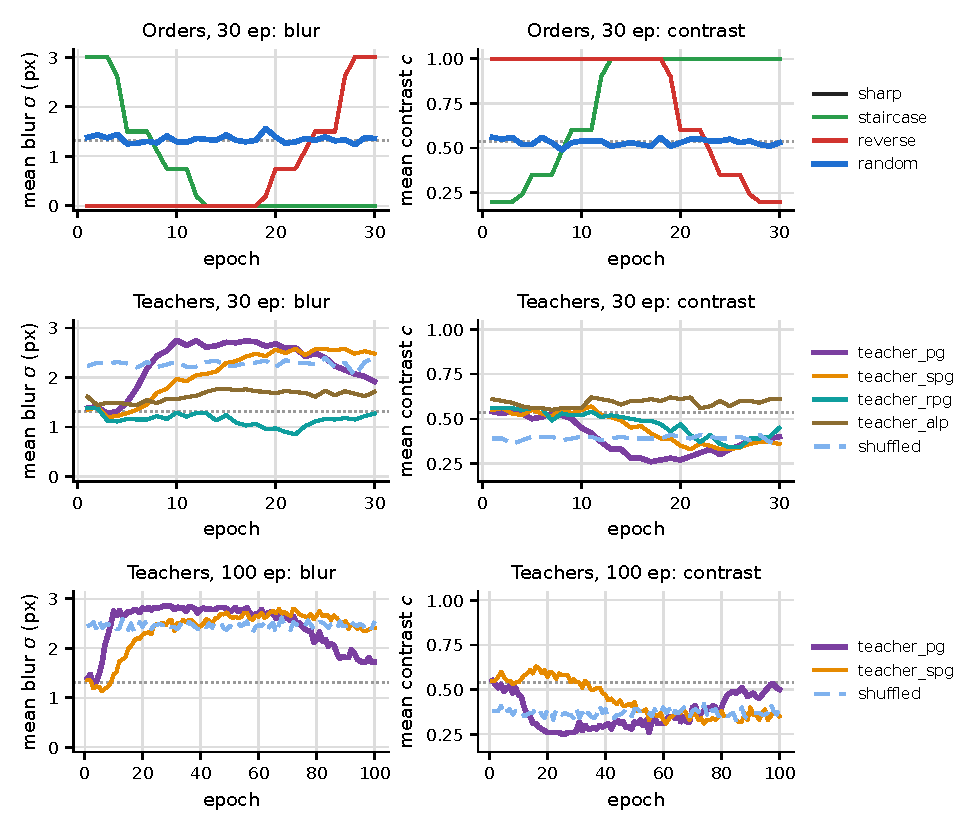
\includegraphics[width=\textwidth]{curves_compact.pdf}
\caption{Mean blur and contrast per epoch (mean of 3 seeds). Top: the fixed orders at 30 epochs (at 100 epochs they have the same shapes, stretched over 100 epochs); \cond{sharp} is partly hidden under \cond{reverse} (blur) and \cond{staircase} (contrast). Middle and bottom: the teachers at 30 and 100 epochs. The staircase starts blurry by design, but no teacher does; PG and SPG drift towards blur and low contrast, and at 100 epochs \cond{teacher\_pg} stays degraded for most of training.}
\label{fig:curves}
\end{figure}

Figure~\ref{fig:worst} shows the share of batches on the most degraded arm $(\sigma=3, c=0.2)$ in each fifth of training. Raw PG piles up there (71--74\% in the middle of a 30-epoch run, up to 83\% at 100 epochs); RPG and ALP-GMM stay at the uniform level (1/16). At 30 epochs, the share in the 3rd / 5th fifth is 0.71 / 0.53 for \cond{teacher\_pg}, 0.38 / 0.65 for \cond{teacher\_spg}, 0.01 / 0.02 for \cond{teacher\_rpg}, 0.27 / 0.45 and 0.82 / 0.17 for $\eta=0.003$ and $0.03$, 0.10 / 0.14 without importance weighting (a slow drift), 0.02 / 0.07 for ALP-GMM (near uniform, slightly harder), 0.45 / 0.46 for \cond{shuffled} and 0.06 / 0.08 for \cond{random}. Changing $\eta$ changes only the speed; both values are still hard-first.

\textbf{Why the hardest arm?} Raw PG is a drop in loss. The loss is highest on the most degraded arm, so one SGD step lowers it most there, and the raw reward is largest. RPG divides by the loss and removes this scale; then the share of the hardest arm falls from 71--74\% (PG) to 1--3\% (RPG). The RPG experiment supports this explanation. We have not yet analysed the per-arm reward distribution directly (the rewards are stored in \texttt{teacher.npz}).

\begin{figure}[htbp]
\centering
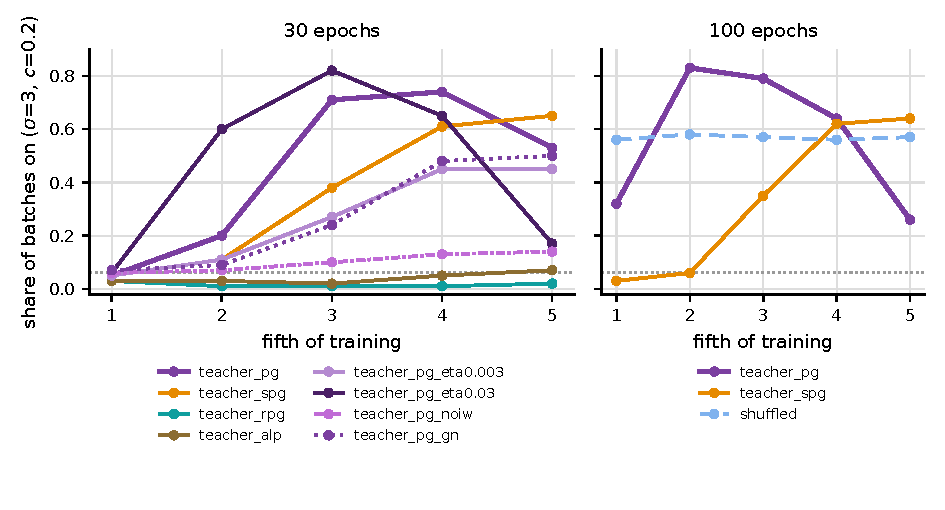
\includegraphics[width=\textwidth]{worst_share.pdf}
\caption{Share of batches on the most degraded arm per fifth of training: raw PG concentrates there, while relative PG and ALP-GMM stay at the uniform level (dotted, 1/16).}
\label{fig:worst}
\end{figure}

\textbf{Three orders: blurry-to-sharp, sharp-to-blurry, random.} \cond{staircase} and \cond{reverse} see exactly the same arms, in opposite time order; \cond{random} sees the full grid, mixed all the time. \textbf{Blurry-to-sharp} (\cond{staircase}) keeps clean accuracy (93.1 at 100 epochs). On C it is better than \cond{sharp} (+3.5 / +3.8) and worse than \cond{random} ($-8.3$ / $-5.6$). On PGD at 100 epochs it is the highest: 57.8 $\pm$ 0.1 vs 56.6 $\pm$ 0.5 for \cond{random}. \textbf{Sharp-to-blurry} (\cond{reverse}) sees blur in the last epochs, so C-seen is high (80.9). But clean drops (86.0), C-unseen is the worst (71.9), and PGD collapses (18.6, 26 points below \cond{sharp}). \textbf{Random} is clearly the best on C, and only 0.9 points below \cond{staircase} on clean. So the direction matters: \cond{reverse} is clearly worse. But blurry-to-sharp is not better than seeing the same kinds of arms mixed.

\textbf{Which axis and which regime?} The 30-epoch ablations isolate the axis and the training regime (Table~\ref{tab:full30}). \textbf{The blur axis gives the robustness:} \cond{random\_blur} reaches 82.1 / 81.9 on C, the same as \cond{random}; \cond{random\_contrast} reaches 68.2 / 73.6, the same as \cond{sharp}. \textbf{Contrast is learned only per image or without BatchNorm:} on the contrast corruption, \cond{random} per batch gets 69.3 and \cond{random\_image} gets 88.9; \cond{sharp} with BatchNorm gets 73.8 and with GroupNorm 87.6; batch-level \cond{random\_contrast} gets only 76.1. \textbf{Costs:} GroupNorm loses about 3 points of clean accuracy at 30 epochs (90.2 vs 93.2), and \cond{random\_image} has low PGD accuracy (37.0). With GroupNorm, \cond{teacher\_pg} is still hard-first (share of the hardest arm 0.50 in the last fifth). \textbf{Staircase length:} a longer blurry phase gives more robustness and less clean accuracy. Even the 75\% staircase stays below \cond{random} on C (78.9 / 80.3 vs 81.4 / 82.2). This fits an effect of how much blur is seen.

\textbf{Shape bias and adversarial robustness.} Shape bias grows with the time spent on the most degraded arm (Figure~\ref{fig:shape}): \cond{sharp} 6.2, \cond{random} 22.7, \cond{teacher\_pg} 54.2, \cond{shuffled} 59.7 (30 epochs). \cond{shuffled} sees the same arms as \cond{teacher\_pg} without order, and its shape bias is slightly higher. The cost is accuracy on high frequencies: high-pass $\sigma=1$ accuracy is 80.2 for \cond{sharp}, 39.7 for \cond{teacher\_pg} and 35.7 for \cond{shuffled}. Blur helps PGD: \cond{sharp} 34.8, \cond{random} 59.5 (30 epochs). \cond{reverse} is the worst (26.7 / 18.6 at 30 / 100 epochs).

\begin{figure}[htbp]
\centering
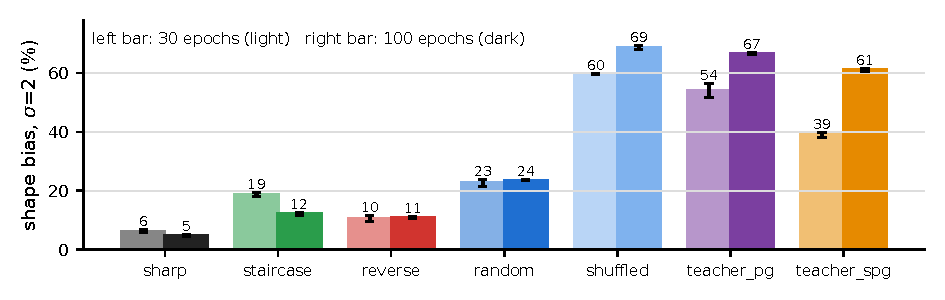
\includegraphics[width=\textwidth]{shape_bias_compact.pdf}
\caption{Shape bias ($\sigma=2$ hybrids) for the main conditions: it follows exposure to heavy blur, not order; \cond{shuffled} (hatched) is at least as high as \cond{teacher\_pg}.}
\label{fig:shape}
\end{figure}

\textbf{How sure are we?} Table~\ref{tab:sure} grades each claim by its evidence.

\begin{table}[htbp]
\caption{Strength of the main claims.}
\label{tab:sure}
\begin{center}
\footnotesize
\renewcommand{\arraystretch}{1.05}
\begin{tabular}{|P{2.1cm}|P{12.2cm}|} \hline
\textbf{Strength} & \textbf{Claim and evidence} \\ \hline
Solid & \textbf{No teacher started blurry.} Seven teacher variants (PG, SPG, RPG, ALP-GMM, two $\eta$ values, no importance weighting) plus PG with GroupNorm, each with 3 seeds. All start near uniform. H1 is rejected in this set-up. \\ \hline
Solid & \textbf{At 100 epochs no order beat \cond{random} on CIFAR-10-C.} \cond{random} 85.3 / 84.4; the closest teacher, \cond{teacher\_spg}, 82.5 / 80.7. The gap is far above the std ($\le$0.9). \\ \hline
Solid & \textbf{Blur gives the robustness, contrast does not.} \cond{random\_blur} $\approx$ \cond{random}; \cond{random\_contrast} $\approx$ \cond{sharp} (30 epochs). \\ \hline
Solid & \textbf{Contrast is learned only per image or with GroupNorm} (88.9 and 87.6 vs 69.3 per batch on the contrast corruption). The BatchNorm mechanism is an explanation; we did not analyse activations. \\ \hline
Fine distinction & \textbf{\cond{teacher\_pg} and \cond{shuffled} are close, not equal.} On robustness the gap is small and favours the teacher: clean +0.6 / +0.8, C-seen +0.4 / +0.6, C-unseen +0.3 / +0.2 (30 / 100 epochs), with std 0.1--0.3, which is weak evidence with 3 seeds. On shape bias and PGD \cond{shuffled} is ahead: shape bias 59.7 vs 54.2 (30 ep) and 68.7 vs 66.6 (100 ep); PGD 51.2 vs 49.3 (30 ep) and 49.3 vs 48.5 (100 ep). The teacher's order adds no measurable robustness, but we cannot say that order never matters. \\ \hline
Fine distinction & \textbf{Direction matters.} \cond{reverse} is clearly the worst order (C-unseen 71.9, PGD 18.6 at 100 epochs). So the claim is ``blurry-to-sharp is not better than mixing'', not ``order is irrelevant''. \\ \hline
Fine distinction & \textbf{``Random is best'' holds among the main seven at 100 epochs on CIFAR-10-C.} At 30 epochs some new variants tie or win in part: \cond{random\_image} 86.9 C-seen (vs 81.4) but 81.2 C-unseen (vs 82.2); \cond{teacher\_rpg} 90.0 / 81.1 / 82.4 $\approx$ \cond{random}; \cond{random\_blur} +1.4 clean, +0.7 C-seen. These were not run at 100 epochs. On PGD at 100 epochs \cond{staircase} is 1.2 points above \cond{random}. \\ \hline
Explanation & \textbf{The teacher goes to the hardest arm because the loss drop is largest there.} Supported by RPG (hard-first disappears when the scale is removed), not by a direct per-arm reward analysis. \\ \hline
\end{tabular}
\end{center}
\end{table}

%======================================================================
\chapter{CONCLUSION}

\textbf{H1 is rejected in our set-up:} no teacher variant started blurry; raw prediction gain sends the teacher to the most degraded arm, where the loss drop is largest, while relative progress and ALP-GMM stay near uniform. \textbf{H2: exposure, not order.} Corruption robustness, PGD robustness and the shape-bias proxy grow with exposure to blur; the teacher's order adds no measurable robustness over the same arms shuffled; a uniform random arm per batch was the best of the seven main conditions on CIFAR-10-C at 100 epochs, though direction matters (Table~\ref{tab:sure}). These results agree with earlier warnings that curriculum gains often come from exposure \cite{wu2021curricula,katzhendler2019} and that mixed blur is a strong baseline \cite{jang2024blur}.

\textbf{Limitations.} (i)~One dataset (CIFAR-10) and one model (ResNet-18); at 32 pixels, $\sigma=3$ blur is very strong. (ii)~Three seeds; differences below 1 point are weak evidence. (iii)~The shape-bias measure is a frequency proxy, not Geirhos' test. (iv)~BatchNorm recalibration is a choice; another fix (for example mixed batches during training) may give different clean numbers. (v)~ALP-GMM samples a continuous space but training rounds to the 16 arms; a continuous version was not tried. (vi)~The \cond{random\_image} arm log stores only the first image's arm (an unbiased but incomplete histogram). (vii)~We did not run the noise tests of Arslan et al.\ \cite{arslan2024noise}; the CIFAR-10-C noise corruptions are only a close match.

\textbf{Future work.} (i)~Run \cond{random\_image}, \cond{random\_blur}, \cond{teacher\_rpg} and \cond{teacher\_alp} at 100 epochs (about 40 minutes on an A100) to test ``random is best'' against them. (ii)~A per-image teacher (a distribution over arms for each batch), to combine the contrast benefit of per-image mixing with a teacher. (iii)~A transfer-progress reward: the loss drop on a clean (sharp) validation batch. It steers the teacher to the arm that helps sharp vision most, not where loss falls most; robustness still stays out of the reward. (iv)~A per-arm reward analysis from \texttt{teacher.npz}, to test the hard-first explanation directly. (v)~A larger dataset (for example Tiny-ImageNet), if the budget allows.

\bibliographystyle{styles/fbe_tez_v11}
\bibliography{references}

\appendix
\chapter{FULL RESULT TABLES AND EXPERIMENT LOG}

Mean $\pm$ std over 3 seeds, in \%. Noise: mean of the 4 noise corruptions. C-contr.: contrast corruption. Shape: hybrid shape bias at $\sigma=2$. HP $\sigma$1: high-pass accuracy at $\sigma=1$. PGD: PGD-10 at $\epsilon=1/255$ on 2\,000 test images. Source: the result summaries (\texttt{results/\{short,full\}\_summary.json}), as copied into \texttt{docs/reports/pilot-short-s0.html}. Table~\ref{tab:log} summarises the experiment log; the full log is in \texttt{docs/experiments.md}.

\begin{table}[htbp]
\caption{All 20 conditions at 30 epochs.}
\label{tab:full30}
\begin{center}
\footnotesize
\setlength{\tabcolsep}{1.6pt}
\begin{tabular}{lcccccccc}
\hline
Condition & Clean & C-seen & C-unseen & Noise & C-contr. & Shape & HP $\sigma$1 & PGD \\
\hline
\texttt{sharp} & $93.2{\scriptstyle\,\pm0.1}$ & $69.6{\scriptstyle\,\pm0.4}$ & $73.3{\scriptstyle\,\pm0.1}$ & $55.5{\scriptstyle\,\pm0.1}$ & $73.8{\scriptstyle\,\pm0.6}$ & $6.2{\scriptstyle\,\pm0.4}$ & $80.2{\scriptstyle\,\pm0.8}$ & $34.8{\scriptstyle\,\pm0.6}$ \\
\texttt{staircase} & $90.7{\scriptstyle\,\pm0.2}$ & $75.8{\scriptstyle\,\pm0.7}$ & $78.7{\scriptstyle\,\pm0.0}$ & $68.3{\scriptstyle\,\pm0.4}$ & $68.8{\scriptstyle\,\pm0.4}$ & $18.8{\scriptstyle\,\pm0.7}$ & $65.7{\scriptstyle\,\pm1.2}$ & $55.0{\scriptstyle\,\pm0.5}$ \\
\texttt{reverse} & $84.4{\scriptstyle\,\pm0.2}$ & $78.1{\scriptstyle\,\pm0.1}$ & $71.3{\scriptstyle\,\pm0.8}$ & $55.0{\scriptstyle\,\pm2.4}$ & $74.1{\scriptstyle\,\pm0.4}$ & $10.5{\scriptstyle\,\pm1.0}$ & $75.0{\scriptstyle\,\pm0.5}$ & $26.7{\scriptstyle\,\pm1.2}$ \\
\texttt{random} & $89.4{\scriptstyle\,\pm0.2}$ & $81.4{\scriptstyle\,\pm0.3}$ & $82.2{\scriptstyle\,\pm0.1}$ & $76.4{\scriptstyle\,\pm0.1}$ & $69.3{\scriptstyle\,\pm0.8}$ & $22.7{\scriptstyle\,\pm1.2}$ & $66.1{\scriptstyle\,\pm2.4}$ & $59.5{\scriptstyle\,\pm1.0}$ \\
\texttt{shuffled} & $84.2{\scriptstyle\,\pm0.3}$ & $79.7{\scriptstyle\,\pm0.2}$ & $78.5{\scriptstyle\,\pm0.1}$ & $75.4{\scriptstyle\,\pm0.2}$ & $63.7{\scriptstyle\,\pm0.5}$ & $59.7{\scriptstyle\,\pm0.1}$ & $35.7{\scriptstyle\,\pm0.9}$ & $51.2{\scriptstyle\,\pm0.1}$ \\
\texttt{teacher\_pg} & $84.8{\scriptstyle\,\pm0.3}$ & $80.1{\scriptstyle\,\pm0.2}$ & $78.8{\scriptstyle\,\pm0.2}$ & $74.8{\scriptstyle\,\pm0.3}$ & $64.1{\scriptstyle\,\pm0.3}$ & $54.2{\scriptstyle\,\pm2.4}$ & $39.7{\scriptstyle\,\pm1.5}$ & $49.3{\scriptstyle\,\pm0.9}$ \\
\texttt{teacher\_spg} & $87.0{\scriptstyle\,\pm0.1}$ & $81.0{\scriptstyle\,\pm0.2}$ & $80.3{\scriptstyle\,\pm0.1}$ & $75.4{\scriptstyle\,\pm0.3}$ & $66.3{\scriptstyle\,\pm0.9}$ & $39.0{\scriptstyle\,\pm0.8}$ & $52.9{\scriptstyle\,\pm1.0}$ & $54.0{\scriptstyle\,\pm0.1}$ \\
\texttt{teacher\_rpg} & $90.0{\scriptstyle\,\pm0.2}$ & $81.1{\scriptstyle\,\pm0.4}$ & $82.4{\scriptstyle\,\pm0.1}$ & $76.3{\scriptstyle\,\pm0.6}$ & $70.5{\scriptstyle\,\pm0.6}$ & $17.6{\scriptstyle\,\pm1.9}$ & $66.4{\scriptstyle\,\pm1.9}$ & $58.0{\scriptstyle\,\pm0.9}$ \\
\texttt{teacher\_pg\_eta0.003} & $86.6{\scriptstyle\,\pm0.0}$ & $81.1{\scriptstyle\,\pm0.1}$ & $80.2{\scriptstyle\,\pm0.2}$ & $75.5{\scriptstyle\,\pm0.5}$ & $66.1{\scriptstyle\,\pm0.5}$ & $44.2{\scriptstyle\,\pm1.0}$ & $49.2{\scriptstyle\,\pm1.5}$ & $53.3{\scriptstyle\,\pm1.3}$ \\
\texttt{teacher\_pg\_eta0.03} & $84.6{\scriptstyle\,\pm0.3}$ & $79.9{\scriptstyle\,\pm0.2}$ & $78.8{\scriptstyle\,\pm0.2}$ & $75.5{\scriptstyle\,\pm0.3}$ & $64.1{\scriptstyle\,\pm0.7}$ & $55.7{\scriptstyle\,\pm1.8}$ & $38.4{\scriptstyle\,\pm3.6}$ & $51.3{\scriptstyle\,\pm0.4}$ \\
\texttt{teacher\_pg\_noiw} & $88.8{\scriptstyle\,\pm0.1}$ & $81.6{\scriptstyle\,\pm0.2}$ & $81.7{\scriptstyle\,\pm0.0}$ & $75.9{\scriptstyle\,\pm0.1}$ & $68.8{\scriptstyle\,\pm0.4}$ & $28.4{\scriptstyle\,\pm0.2}$ & $61.6{\scriptstyle\,\pm1.5}$ & $59.7{\scriptstyle\,\pm0.8}$ \\
\texttt{teacher\_alp} & $89.0{\scriptstyle\,\pm0.5}$ & $82.1{\scriptstyle\,\pm0.1}$ & $82.0{\scriptstyle\,\pm0.4}$ & $76.4{\scriptstyle\,\pm0.8}$ & $67.7{\scriptstyle\,\pm0.8}$ & $29.9{\scriptstyle\,\pm0.5}$ & $61.3{\scriptstyle\,\pm1.5}$ & $56.6{\scriptstyle\,\pm1.1}$ \\
\texttt{random\_image} & $89.6{\scriptstyle\,\pm0.0}$ & $86.9{\scriptstyle\,\pm0.1}$ & $81.2{\scriptstyle\,\pm0.2}$ & $71.7{\scriptstyle\,\pm0.7}$ & $88.9{\scriptstyle\,\pm0.1}$ & $22.3{\scriptstyle\,\pm0.8}$ & $81.8{\scriptstyle\,\pm0.1}$ & $37.0{\scriptstyle\,\pm1.0}$ \\
\texttt{random\_blur} & $90.8{\scriptstyle\,\pm0.3}$ & $82.1{\scriptstyle\,\pm0.3}$ & $81.9{\scriptstyle\,\pm0.2}$ & $73.8{\scriptstyle\,\pm0.1}$ & $67.2{\scriptstyle\,\pm0.6}$ & $23.3{\scriptstyle\,\pm1.2}$ & $66.8{\scriptstyle\,\pm0.9}$ & $56.4{\scriptstyle\,\pm0.5}$ \\
\texttt{random\_contrast} & $92.7{\scriptstyle\,\pm0.2}$ & $68.2{\scriptstyle\,\pm0.3}$ & $73.6{\scriptstyle\,\pm0.3}$ & $57.4{\scriptstyle\,\pm1.1}$ & $76.1{\scriptstyle\,\pm1.0}$ & $4.2{\scriptstyle\,\pm0.1}$ & $81.6{\scriptstyle\,\pm1.5}$ & $31.2{\scriptstyle\,\pm1.2}$ \\
\texttt{sharp\_gn} & $90.2{\scriptstyle\,\pm0.3}$ & $79.6{\scriptstyle\,\pm0.4}$ & $78.8{\scriptstyle\,\pm0.5}$ & $69.4{\scriptstyle\,\pm1.4}$ & $87.6{\scriptstyle\,\pm0.6}$ & $14.6{\scriptstyle\,\pm1.4}$ & $72.9{\scriptstyle\,\pm0.9}$ & $38.2{\scriptstyle\,\pm1.5}$ \\
\texttt{random\_gn} & $84.7{\scriptstyle\,\pm0.2}$ & $83.0{\scriptstyle\,\pm0.2}$ & $79.7{\scriptstyle\,\pm0.1}$ & $76.2{\scriptstyle\,\pm0.1}$ & $84.8{\scriptstyle\,\pm0.2}$ & $41.1{\scriptstyle\,\pm1.6}$ & $70.7{\scriptstyle\,\pm1.2}$ & $49.4{\scriptstyle\,\pm0.3}$ \\
\texttt{teacher\_pg\_gn} & $79.0{\scriptstyle\,\pm0.3}$ & $78.3{\scriptstyle\,\pm0.3}$ & $74.6{\scriptstyle\,\pm0.3}$ & $72.3{\scriptstyle\,\pm0.4}$ & $79.4{\scriptstyle\,\pm0.3}$ & $59.3{\scriptstyle\,\pm0.8}$ & $60.7{\scriptstyle\,\pm1.2}$ & $43.2{\scriptstyle\,\pm0.6}$ \\
\texttt{staircase\_f025} & $92.0{\scriptstyle\,\pm0.1}$ & $71.0{\scriptstyle\,\pm0.9}$ & $74.8{\scriptstyle\,\pm0.4}$ & $58.9{\scriptstyle\,\pm1.1}$ & $71.9{\scriptstyle\,\pm0.1}$ & $9.6{\scriptstyle\,\pm0.3}$ & $76.9{\scriptstyle\,\pm0.6}$ & $41.0{\scriptstyle\,\pm0.8}$ \\
\texttt{staircase\_f075} & $88.5{\scriptstyle\,\pm0.1}$ & $78.9{\scriptstyle\,\pm0.1}$ & $80.3{\scriptstyle\,\pm0.2}$ & $75.0{\scriptstyle\,\pm0.2}$ & $64.5{\scriptstyle\,\pm0.8}$ & $33.2{\scriptstyle\,\pm0.8}$ & $50.8{\scriptstyle\,\pm3.8}$ & $56.1{\scriptstyle\,\pm0.7}$ \\
\hline
\end{tabular}

\end{center}
\end{table}

\begin{table}[htbp]
\caption{The seven main conditions at 100 epochs.}
\label{tab:full100}
\begin{center}
\footnotesize
\setlength{\tabcolsep}{1.6pt}
\begin{tabular}{lcccccccc}
\hline
Condition & Clean & C-seen & C-unseen & Noise & C-contr. & Shape & HP $\sigma$1 & PGD \\
\hline
\texttt{sharp} & $94.8{\scriptstyle\,\pm0.0}$ & $73.5{\scriptstyle\,\pm0.9}$ & $75.0{\scriptstyle\,\pm0.5}$ & $54.3{\scriptstyle\,\pm1.3}$ & $76.1{\scriptstyle\,\pm0.3}$ & $4.7{\scriptstyle\,\pm0.2}$ & $85.0{\scriptstyle\,\pm0.2}$ & $44.9{\scriptstyle\,\pm0.2}$ \\
\texttt{staircase} & $93.1{\scriptstyle\,\pm0.2}$ & $77.0{\scriptstyle\,\pm0.8}$ & $78.8{\scriptstyle\,\pm0.6}$ & $64.0{\scriptstyle\,\pm1.6}$ & $71.5{\scriptstyle\,\pm0.2}$ & $12.2{\scriptstyle\,\pm0.5}$ & $75.7{\scriptstyle\,\pm0.4}$ & $57.8{\scriptstyle\,\pm0.1}$ \\
\texttt{reverse} & $86.0{\scriptstyle\,\pm0.2}$ & $80.9{\scriptstyle\,\pm0.3}$ & $71.9{\scriptstyle\,\pm0.7}$ & $52.1{\scriptstyle\,\pm2.1}$ & $74.4{\scriptstyle\,\pm0.4}$ & $10.9{\scriptstyle\,\pm0.3}$ & $74.9{\scriptstyle\,\pm1.5}$ & $18.6{\scriptstyle\,\pm2.0}$ \\
\texttt{random} & $92.2{\scriptstyle\,\pm0.0}$ & $85.3{\scriptstyle\,\pm0.2}$ & $84.4{\scriptstyle\,\pm0.1}$ & $76.7{\scriptstyle\,\pm0.2}$ & $72.9{\scriptstyle\,\pm0.7}$ & $23.5{\scriptstyle\,\pm0.2}$ & $65.9{\scriptstyle\,\pm1.1}$ & $56.6{\scriptstyle\,\pm0.5}$ \\
\texttt{shuffled} & $85.4{\scriptstyle\,\pm0.1}$ & $80.9{\scriptstyle\,\pm0.1}$ & $79.5{\scriptstyle\,\pm0.1}$ & $76.7{\scriptstyle\,\pm0.4}$ & $63.1{\scriptstyle\,\pm0.9}$ & $68.7{\scriptstyle\,\pm0.8}$ & $27.6{\scriptstyle\,\pm4.8}$ & $49.3{\scriptstyle\,\pm1.2}$ \\
\texttt{teacher\_pg} & $86.2{\scriptstyle\,\pm0.1}$ & $81.5{\scriptstyle\,\pm0.2}$ & $79.7{\scriptstyle\,\pm0.1}$ & $76.1{\scriptstyle\,\pm0.6}$ & $63.6{\scriptstyle\,\pm0.4}$ & $66.6{\scriptstyle\,\pm0.4}$ & $26.9{\scriptstyle\,\pm0.1}$ & $48.5{\scriptstyle\,\pm0.6}$ \\
\texttt{teacher\_spg} & $87.1{\scriptstyle\,\pm0.2}$ & $82.5{\scriptstyle\,\pm0.3}$ & $80.7{\scriptstyle\,\pm0.1}$ & $76.7{\scriptstyle\,\pm0.3}$ & $65.8{\scriptstyle\,\pm0.8}$ & $61.2{\scriptstyle\,\pm0.5}$ & $34.4{\scriptstyle\,\pm1.2}$ & $46.9{\scriptstyle\,\pm1.0}$ \\
\hline
\end{tabular}

\end{center}
\end{table}

\begin{table}[htbp]
\caption{Experiment log (2026).}
\label{tab:log}
\begin{center}
\scriptsize
\renewcommand{\arraystretch}{1.15}
\begin{tabular}{|c|c|P{3.8cm}|P{7.8cm}|} \hline
\textbf{\#} & \textbf{Date} & \textbf{Trial} & \textbf{Result} \\ \hline
1 & 11-03 & Sharp, 30 ep, seed 0 & Clean 93.2\% (target $\sim$93). \\
2 & 11-03 & Eager vs \texttt{torch.compile} & 2.0 vs 1.7 s/epoch; compile costs 30\,s; eager chosen. \\
3 & 11-03 & Pilot: 7 conditions, seed 0 & Mixed conditions 13--60\% clean; BatchNorm suspected. \\
4 & 11-03 & BN recalibration & Confirmed: \cond{random} 60$\to$89, \cond{teacher\_spg} 16$\to$87 clean. \\
5 & 11-04 & F5: 7 $\times$ 3 $\times$ 30 ep & \cond{random} best on C; teacher goes to the hardest arm. \\
6 & 11-08 & F6: 7 $\times$ 3 $\times$ 100 ep & Same ranking as F5. \\
7 & 11-08 & \cond{teacher\_rpg} & Hardest-arm share 1--3\% (PG: 71--74\%); $\approx$ \cond{random}. \\
8 & 11-08 & $\eta$ 0.003 / 0.03 & Only speed changes; both still hard-first. \\
9 & 11-08 & No importance weighting & Slow drift (14\% late). \\
10 & 11-08 & ALP-GMM & Near uniform, slightly harder; $\approx$ \cond{random}. \\
11 & 11-08 & Random arm per image & Contrast corruption 88.9 (per batch 69.3); PGD low (37.0). \\
12 & 11-08 & GroupNorm & \cond{sharp\_gn} contrast 87.6 (BN 73.8); clean $-3$; teacher still hard-first. \\
13 & 11-08 & Blur-only / contrast-only & Blur $\approx$ \cond{random}; contrast-only $\approx$ \cond{sharp}. \\
14 & 11-08 & Staircase 25\% / 75\% & Longer blurry phase: more robust, less clean. \\
15 & 11-08 & Shape bias, low/high-pass & Follows blur exposure, not order. \\
16 & 11-08 & FGSM, PGD-10 & Blur helps PGD; FGSM likely gradient-masked, not used. \\
17 & 11-08 & OOM at 12 parallel runs & 3 runs re-run at 6 parallel from checkpoint. \\ \hline
\end{tabular}
\end{center}
\end{table}

\end{document}
